\documentclass{article}
\usepackage{tikz}
\usetikzlibrary{trees}

\begin{document}

    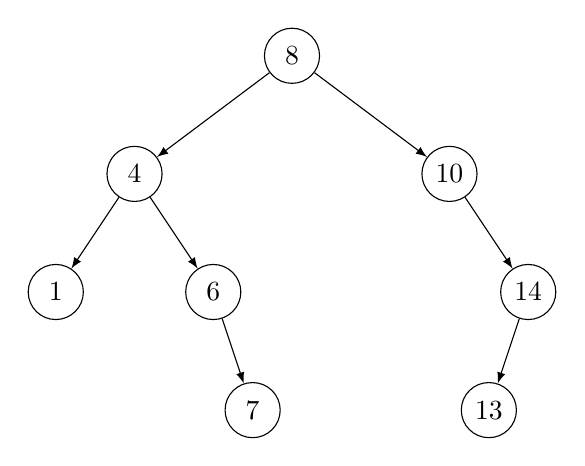
\begin{tikzpicture}[
        grow=down,
        level 1/.style = {sibling distance=4cm},        level 2/.style = {sibling distance=2cm},        level 3/.style = {sibling distance=1cm},        level 4/.style = {sibling distance=0.5cm},        level distance=1.5cm,
        every node/.style={circle, draw, minimum size=7mm, inner sep=2pt},
        edge from parent/.style={draw, -latex}
    ]
 \node {8}
     child {  node {4}
     child {  node {1} }
     child {  node {6}
     child [missing]
     child {  node {7} } } }
     child {  node {10}
     child [missing]
     child {  node {14}
     child {  node {13} }
     child [missing] } };
    \end{tikzpicture}

\end{document}
